\chapter{Emissioni radiate}
L'obiettivo prioritario nello studio delle emissioni radiate risiede nel controllo delle \textbf{sorgenti non intenzionali} di campi elettromagnetici. A differenza delle emissioni intenzionali, in cui la struttura radiante è ottimizzata per trasmettere o ricevere energia elettromagnetica a frequenze determinate, qualsiasi circuito percorso da correnti variabili nel tempo si comporta potenzialmente come un'antenna parassita non intenzionale.
\begin{figure}[H]
	\centering
	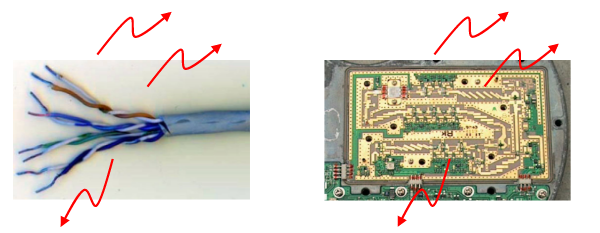
\includegraphics[width=0.6\linewidth]{immagini/emissioni_radiate1}
\end{figure}

In linea di principio, il campo elettromagnetico irradiato si propaga in tutte le direzioni dello spazio. Tale propagazione è perturbata dai fenomeni di riflessione generati da qualsiasi ostacolo presente nell'ambiente, con particolare criticità in presenza di strutture metalliche; questo fenomeno, denominato \textbf{scattering}, rende la quantificazione e la riproducibilità del campo radiato estremamente complesse e dipendenti dalla geometria dell'ambiente di misura.

Le equazioni dell'elettromagnetismo ammettono soluzioni progressive che si propagano alla velocità della luce nel mezzo, definita da:
\[
v = \frac{1}{\sqrt{\varepsilon \mu}}
\]
che nel vuoto assume il valore di riferimento:
\[
v = c \approx 3 \cdot 10^8\ \text{m/s}
\]
A seconda della geometria della sorgente e della distanza di osservazione, le onde elettromagnetiche si sviluppano secondo fronti d'onda cilindrici, sferici o localmente piani.
\begin{figure}[H]
	\centering
	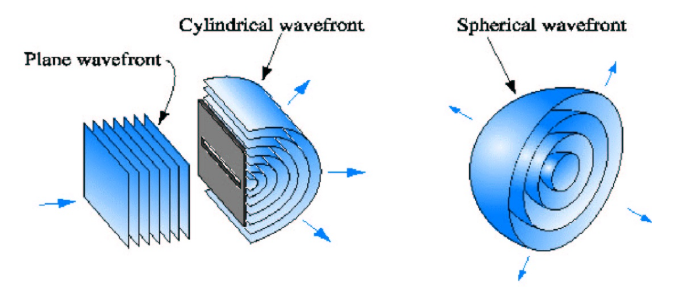
\includegraphics[width=0.55\linewidth]{immagini/emissioni_radiate2}
\end{figure}

L'antenna costituisce l'elemento di transizione tra la propagazione guidata lungo una linea di trasmissione e la propagazione libera nello spazio tridimensionale. La catena di trasmissione radiata si articola nella sequenza seguente:
\begin{enumerate}
    \item Generazione del segnale da parte del circuito trasmettitore.
    \item Propagazione guidata lungo la linea di trasmissione o guida d'onda verso l'antenna trasmittente.
    \item Irradiazione dell'onda elettromagnetica nello spazio libero da parte dell'antenna trasmittente.
    \item Intercettazione dell'onda elettromagnetica da parte dell'antenna ricevente.
    \item Propagazione guidata verso il carico o circuito ricevitore.
\end{enumerate}
\begin{figure}[H]
	\centering
	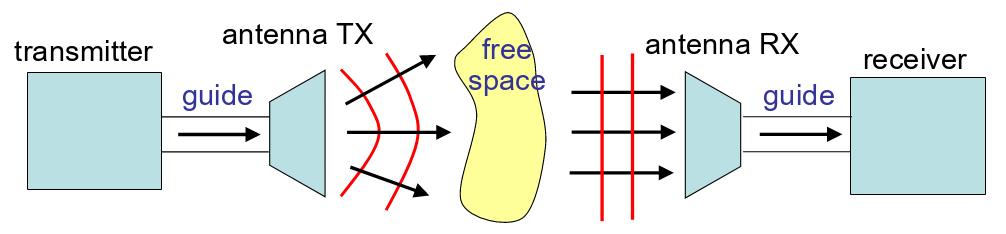
\includegraphics[width=0.7\linewidth]{immagini/emissioni_radiate3}
\end{figure}

Le proprietà delle antenne sono descritte mediante due categorie di parametri:
\begin{figure}[H]
	\centering
	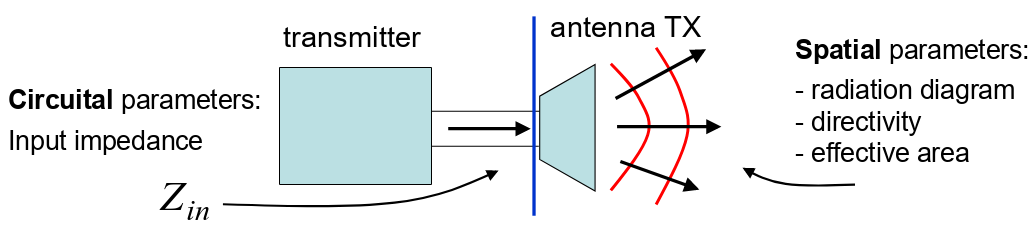
\includegraphics[width=0.6\linewidth]{immagini/emissioni_radiate4}
\end{figure}
\begin{itemize}
    \item \textbf{Parametri circuitali} $\rightarrow$ quantificano il comportamento ai morsetti dell'antenna mediante l'impedenza d'ingresso:
    \[
    Z_{\text{in}} = R_{\text{in}} + j X_{\text{in}} = R_{\text{irr}} + j X_{\text{ant}}
    \]
    dove $R_{\text{irr}}$ rappresenta la resistenza di radiazione, indice della capacità di convertire energia elettrica in campo elettromagnetico radiato nello spazio secondo la potenza attiva dissipata:
    \[
    P = R_{\text{irr}} I^2
    \]
    mentre $X_{\text{ant}}$ rappresenta la reattanza ai morsetti, indice del disadattamento reattivo.
    \begin{figure}[H]
    	\centering
    	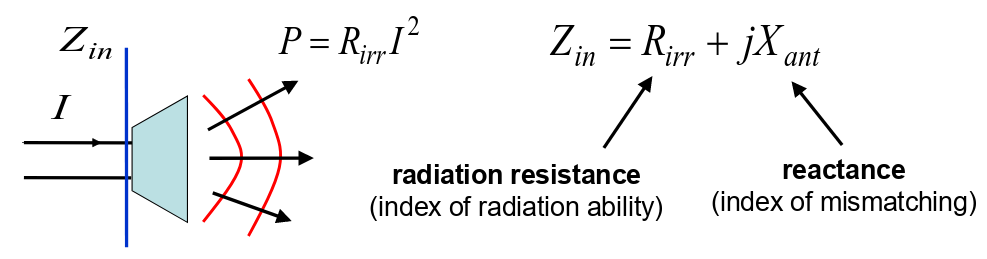
\includegraphics[width=0.6\linewidth]{immagini/emissioni_radiate5}
    \end{figure}
    I parametri circuitali vengono descritti mediante modelli a parametri concentrati.
    \item \textbf{Parametri spaziali} $\rightarrow$ descrivono le proprietà di orientamento spaziale dell'irradiazione, articolandosi in:
    \begin{itemize}
        \item \textbf{Diagramma di radiazione} $\rightarrow$ funzione tridimensionale che descrive la distribuzione angolare della densità di potenza irradiata in funzione delle coordinate sferiche $(\theta, \phi)$.
        \begin{figure}[H]
        	\centering
        	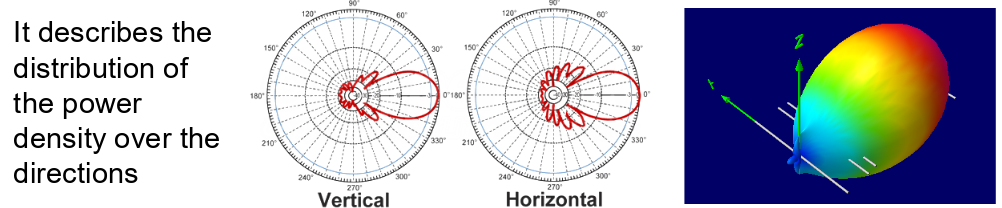
\includegraphics[width=0.6\linewidth]{immagini/emissioni_radiate6}
        \end{figure}
        \item \textbf{Direttività} $\rightarrow$ misura della concentrazione della potenza irradiata in una direzione preferenziale rispetto a un radiatore isotropo.
        \item \textbf{Area efficace} $\rightarrow$ parametro che correla la densità di potenza incidente alla potenza resa disponibile ai morsetti di carico dell'antenna in ricezione.
    \end{itemize}
    I parametri spaziali per essere modellati necessitano della risoluzione delle equazioni di Maxwell (full-wave).
\end{itemize}

Le geometrie delle antenne presentano un'ampia diversificazione in termini di frequenza di lavoro, ingombri fisici e livelli di potenza gestiti. Tra le principali tipologie figurano:
\begin{itemize}
    \item Schiere di dipoli (array Yagi-Uda).
    \item Antenne a elica.
    \item Schiere lineari per radiotelescopi.
    \item Antenne a microstriscia (patch antenna) integrate su circuito stampato.
\end{itemize}
\begin{figure}[H]
	\centering
	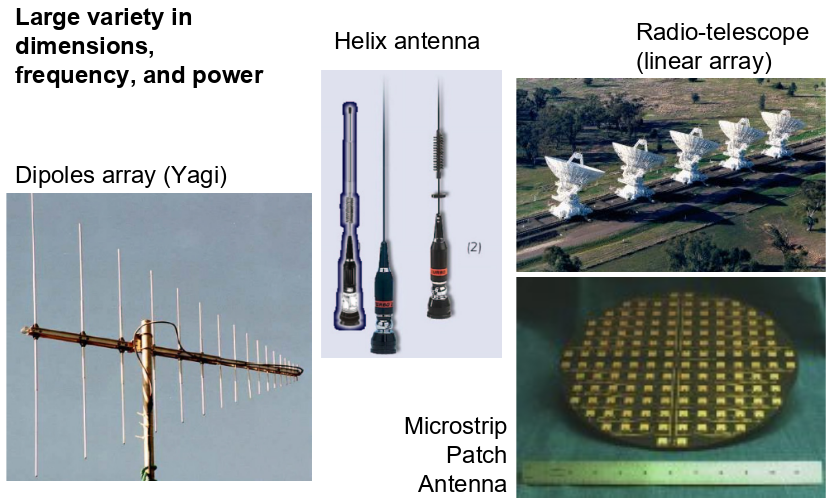
\includegraphics[width=0.7\linewidth]{immagini/emissioni_radiate7}
\end{figure}


\section{Condizioni di campo lontano e ambiente di misura}
La caratterizzazione di una sorgente di disturbo elettromagnetico impone l'individuazione della zona spaziale in cui viene condotta l'indagine. Lo spazio circostante la sorgente viene suddiviso in due regioni fisiche fondamentali:
\begin{itemize}
    \item \textbf{Campo vicino} $\rightarrow$ regione spaziale prossima alla sorgente in cui:
    \begin{itemize}
        \item La struttura del campo è di tipo quasi-statico e non si configura come onda TEM.
        \item Il rapporto tra campo elettrico $\vec{E}$ e campo magnetico $\vec{H}$ non è costante, dipendendo dalla natura circuitale della sorgente (elettrica o magnetica).
        \item La potenza elettromagnetica presenta una componente reattiva non trascurabile.
        \item Le misure risentono della presenza di oggetti metallici e dell'ambiente circostante.
        \item I modelli circuitali semplificati di emissione non risultano applicabili.
    \end{itemize}
    \item \textbf{Campo lontano} $\rightarrow$ regione asintotica a grande distanza dalla sorgente in cui:
    \begin{itemize}
        \item L'onda si propaga con struttura TEM ed è assimilabile localmente a un'onda piana.
        \item Modulo di campo elettrico e magnetico decadono inversamente con la distanza come $1/r$.
        \item Il rapporto tra l'ampiezza del campo elettrico e del campo magnetico è costante e pari all'impedenza intrinseca del mezzo $\zeta$:
        \[
        \frac{|\vec{E}|}{|\vec{H}|} = \zeta = \sqrt{\frac{\mu}{\varepsilon}}
        \]
        \item La potenza trasportata è esclusivamente di tipo attivo (vettore di Poynting reale).
        \item Le misure risultano controllabili, ripetibili e prive delle instabilità di campo vicino.
        \item Risulta possibile impiegare modelli analitici semplificati per la simulazione dei campi.
    \end{itemize}
\end{itemize}

Affinché le condizioni di campo lontano siano verificate rispetto a una sorgente radiante di dimensione massima pari a $d_{\text{max}}$, la distanza di osservazione $r$ deve soddisfare tre vincoli:
\[
r \gg \lambda, \quad r \gg d_{\text{max}}, \quad r \gg \frac{2 d_{\text{max}}^2}{\lambda}
\]
\begin{figure}[H]
	\centering
	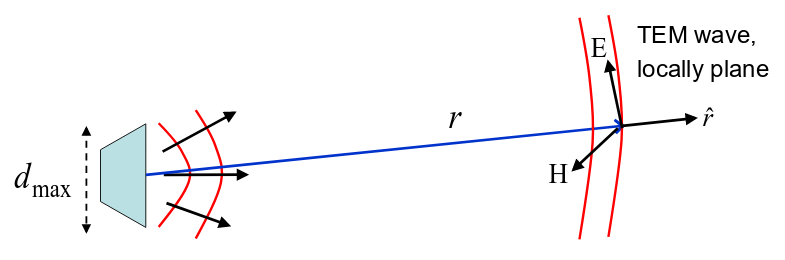
\includegraphics[width=0.6\linewidth]{immagini/emissioni_radiate8}
\end{figure}
Nella zona di campo lontano, campo elettrico e magnetico presentano le seguenti relazioni:
\[
\vec{E} = \frac{e^{-j \beta r}}{r} \vec{e}(\theta, \phi)
\]
\[
\vec{H} = \frac{1}{\zeta} \hat{r} \times \vec{E}
\]
in cui si evidenziano:
\begin{itemize}
    \item \textbf{Fattore comune} $\rightarrow$ termine sferico divergente $\frac{e^{-j \beta r}}{r}$, che governa la fase di propagazione e il decadimento d'ampiezza con la distanza.
    \item \textbf{Fattore di forma} $\rightarrow$ vettore $\vec{e}(\theta, \phi)$, che definisce la dipendenza angolare e la polarizzazione del campo irradiato.
    \item \textbf{Costante di fase} $\rightarrow$ parametro $\beta$, espresso da:
    \[
    \beta = \frac{\omega}{c} = \omega \sqrt{\varepsilon \mu}
    \]
    \item \textbf{Impedenza intrinseca} $\rightarrow$ valore scalare $\zeta = \sqrt{\mu/\varepsilon}$, pari nel vuoto a $\zeta_0 \approx 377\ \Omega$.
\end{itemize}


Le normative internazionali per la certificazione della compatibilità elettromagnetica impongono che le emissioni radiate siano quantificate esclusivamente in condizioni di campo lontano e in assenza di riflessioni ambientali. L'intervallo di frequenza standard è compreso tra $30\text{ MHz}$ ($0.03\text{ GHz}$) e $1\text{ GHz}$, con una frequenza di transizione normata posta a $230\text{ MHz}$ ($0.23\text{ GHz}$).

Le misure vengono eseguite posizionando l'antenna di ricezione a una distanza convenzionale di riferimento pari a $10\text{ m}$ dall'apparato sotto prova (EUT). Il campo elettrico misurato viene espresso in scala logaritmica in decibel microvolt al metro ($\text{dB}\mu\text{V/m}$).

Le soglie limite prescritte dai regolamenti (quali FCC e CISPR) si articolano in due classi distinte:
\begin{itemize}
    \item \textbf{Classe A} $\rightarrow$ destinata ad apparati installati in ambienti industriali e commerciali:
    \begin{itemize}
        \item Da $30\text{ MHz}$ a $230\text{ MHz}$: limite di emissione pari a $40\text{ dB}\mu\text{V/m}$.
        \item Da $230\text{ MHz}$ a $1\text{ GHz}$: limite di emissione pari a $47\text{ dB}\mu\text{V/m}$.
    \end{itemize}
    \item \textbf{Classe B} $\rightarrow$ destinata ad apparati per uso residenziale, civile e domestico (soggetta a vincoli più restrittivi):
    \begin{itemize}
        \item Da $30\text{ MHz}$ a $230\text{ MHz}$: limite di emissione pari a $30\text{ dB}\mu\text{V/m}$.
        \item Da $230\text{ MHz}$ a $1\text{ GHz}$: limite di emissione pari a $37\text{ dB}\mu\text{V/m}$.
    \end{itemize}
\end{itemize}

I limiti normativi a $10\text{ m}$ sono riassunti nella tabella seguente:
\begin{center}
\begin{tabular}{|l|c|c|}
\hline
\textbf{Classe di certificazione} & \textbf{Banda $30 - 230\text{ MHz}$} & \textbf{Banda $230 - 1000\text{ MHz}$} \\
\hline
Classe A (Industriale) & $40\ \text{dB}\mu\text{V/m}$ & $47\ \text{dB}\mu\text{V/m}$ \\
\hline
Classe B (Residenziale) & $30\ \text{dB}\mu\text{V/m}$ & $37\ \text{dB}\mu\text{V/m}$ \\
\hline
\end{tabular}
\end{center}
\begin{figure}[H]
	\centering
	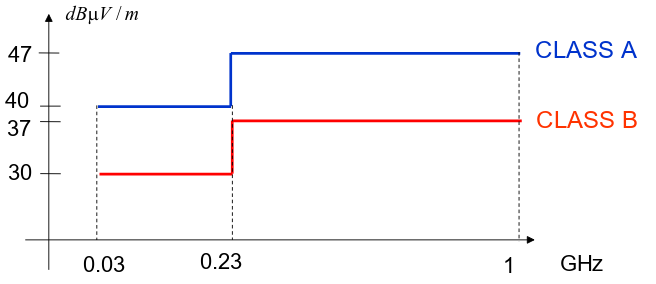
\includegraphics[width=0.6\linewidth]{immagini/emissioni_radiate9}
\end{figure}

Per garantire la riproducibilità e l'accuratezza delle misure, è indispensabile creare un ambiente di propagazione controllato in cui siano garantite le condizioni di campo lontano e l'assoluta assenza di riflessioni parassite. A tale scopo si utilizzano strutture schermate dedicate:
\begin{itemize}
    \item \textbf{Camera anecoica} $\rightarrow$ ambiente completamente schermato verso i campi elettromagnetici esterni mediante pareti metalliche, e internamente rivestito da materiali fonoassorbenti alle radiofrequenze (piramidi in schiuma poliuretanica caricata al carbonio e piastrelle di ferrite) disposti su tutte le pareti, sul soffitto e sul pavimento; garantisce una zona di test a riflessioni trascurabili in cui l'attenuazione e l'uniformità del campo risultano prefissate.
    \item \textbf{Camera semi-anecoica} $\rightarrow$ configurazione in cui le pareti verticali e il soffitto sono rivestiti da materiale assorbente, mentre il pavimento è costituito da un piano metallico perfettamente riflettente; tale configurazione modella in modo fedele la propagazione su suolo reale.
\end{itemize}
\begin{figure}[H]
	\centering
	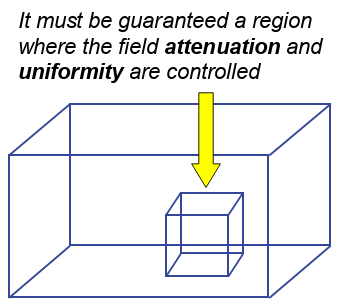
\includegraphics[width=0.3\linewidth]{immagini/emissioni_radiate10}
\end{figure}

A titolo esemplificativo, l'infrastruttura di misura semi-anecoica dell'Università di Cassino e del Lazio Meridionale presenta le seguenti caratteristiche costruttive e dimensionali:
\begin{itemize}
    \item \textbf{Camera semi-anecoica} $\rightarrow$ lunghezza $L_{\text{ca}} = 9060\text{ mm}$, larghezza $l_{\text{ca}} = 5700\text{ mm}$, altezza $h_{\text{ca}} = 6200\text{ mm}$; rivestimento costituito da piastrelle di ferrite con passo $30 \times 30\text{ cm}$ associate a coni in materiale assorbente.
    \item \textbf{Camera di controllo schermata} $\rightarrow$ lunghezza $L_{\text{cc}} = 5000\text{ mm}$, larghezza $l_{\text{cc}} = 3150\text{ mm}$, altezza $h_{\text{cc}} = 2900\text{ mm}$; rivestimento con doppio strato di pannelli metallici continui.
\end{itemize}
\begin{figure}[H]
	\centering
	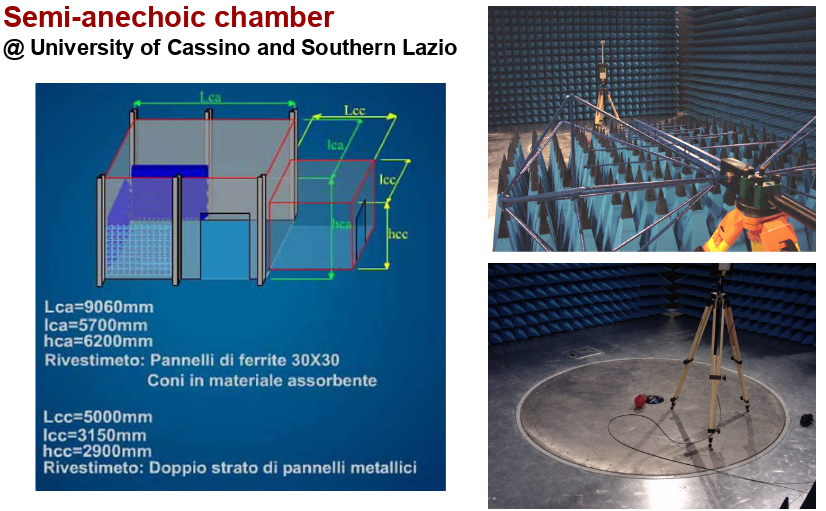
\includegraphics[width=0.7\linewidth]{immagini/emissioni_radiate11}
\end{figure}

\section{Modellazione delle emissioni radiate}
La sorgente fondamentale di emissione non intenzionale nei circuiti stampati è rappresentata da una coppia di conduttori paralleli.

Nel dominio della frequenza, la conoscenza della distribuzione spaziale di corrente $I(z)$ lungo il conduttore orientato lungo l'asse $z$ è indispensabile. Indicando con $I_0$ l'ampiezza di riferimento e con $f(z)$ il profilo di distribuzione spaziale normalizzato ($I(z) = I_0 f(z)$), il campo elettrico radiato in campo lontano assume la forma:
\[
\vec{E} = I_0 \frac{e^{-j \beta r}}{r} \vec{e}(\theta, \phi)
\]
dove $\vec{e}(\theta, \phi)$ costituisce il fattore di forma associato alla geometria della linea e alla distribuzione di corrente $f(z)$.
\begin{figure}[H]
	\centering
	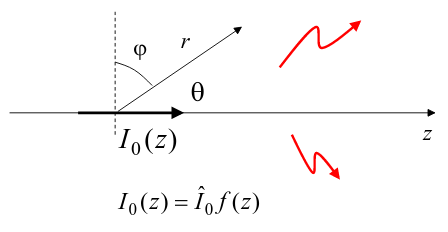
\includegraphics[width=0.4\linewidth]{immagini/emissioni_radiate13}
\end{figure}

Nel caso di una coppia di conduttori rettilinei paralleli separati da una distanza $d$, il campo totale in un punto di osservazione di campo lontano viene ricavato per sovrapposizione lineare dei singoli contributi radiativi, secondo il principio dell'array di due antenne elementari:
\[
\vec{E} = \vec{e}(\theta, \phi) \left[ I_{01} \frac{e^{-j \beta r_1}}{r_1} + I_{02} \frac{e^{-j \beta r_2}}{r_2} \right]
\]
dove $r_1$ ed $r_2$ indicano le distanze geometriche dai singoli conduttori al punto di campo, mentre $I_{01}$ e $I_{02}$ rappresentano le rispettive correnti d'ingresso.
\begin{figure}[H]
	\centering
	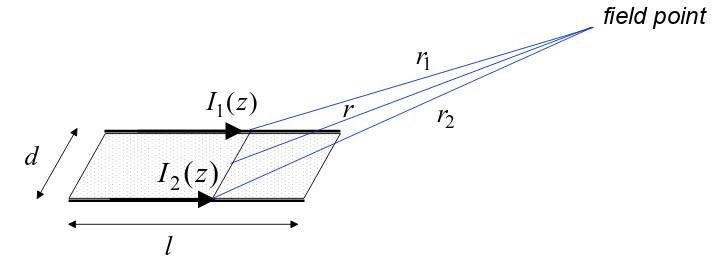
\includegraphics[width=0.6\linewidth]{immagini/emissioni_radiate14}
\end{figure}
Nelle condizioni di campo lontano ($r \gg d$), si introducono le consuete approssimazioni:
\begin{itemize}
    \item \textbf{Approssimazione in ampiezza} $\rightarrow$ al denominatore la differenza di percorso ha un effetto trascurabile sull'attenuazione $1/r$:
    \[
    r_1 \approx r_2 \approx r
    \]
    \item \textbf{Approssimazione in fase} $\rightarrow$ all'esponente (fase) la differenza di cammino ottico modifica sensibilmente l'interferenza tra i contributi:
    \[
    r_1 \approx r + \Delta r, \quad r_2 \approx r - \Delta r
    \]
\end{itemize}
Dalla proiezione trigonometrica della geometria dell'array rispetto alle coordinate sferiche, la variazione di cammino $\Delta r$ vale:
\[
\Delta r = \frac{d}{2} \sin\phi \sin\theta
\]
\begin{figure}[H]
	\centering
	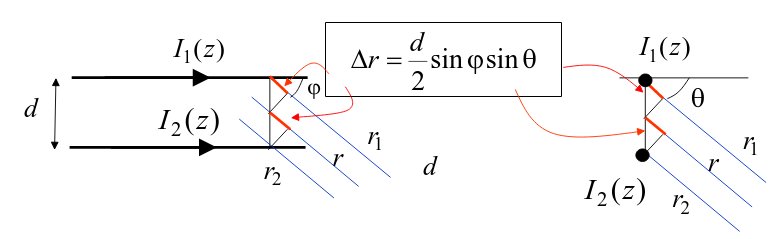
\includegraphics[width=0.6\linewidth]{immagini/emissioni_radiate15}
\end{figure}
Il corrispondente sfasamento elettrico $\beta \Delta r$ è dato da:
\[
\beta \Delta r = \frac{\omega}{c} \frac{d}{2} \sin\phi \sin\theta = \pi \frac{d}{\lambda} \sin\phi \sin\theta
\]

Sostituendo tali approssimazioni, l'espressione generale del campo elettrico radiato dalla coppia di conduttori diventa:
\[
\vec{E} = \vec{e}(\theta, \phi) \frac{e^{-j \beta r}}{r} \left[ I_{01} e^{-j \beta \Delta r} + I_{02} e^{j \beta \Delta r} \right]
\]

La distribuzione di corrente lungo la coppia di linee viene decomposta nelle componenti canoniche di modo:
\begin{itemize}
    \item \textbf{Modo differenziale} $\rightarrow$ le correnti sui due conduttori fluiscono in direzioni opposte con modulo identico:
    \[
    I_1(z) = -I_2(z) = I_D(z) \implies I_{01} = I_{D0}, \quad I_{02} = -I_{D0}
    \]
    \item \textbf{Modo comune} $\rightarrow$ le correnti sui due conduttori fluiscono nella stessa direzione con identica ampiezza e fase:
    \[
    I_1(z) = I_2(z) = I_C(z) \implies I_{01} = I_{C0}, \quad I_{02} = I_{C0}
    \]
\end{itemize}

\subsection{Emissione radiata di modo differenziale}
Nel regime di modo differenziale, le correnti di andata e ritorno sono uguali e contrarie ($I_{01} = I_{D0}$, $I_{02} = -I_{D0}$). 
\begin{figure}[H]
	\centering
	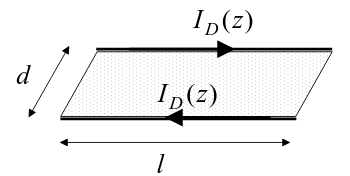
\includegraphics[width=0.3\linewidth]{immagini/emissioni_radiate16}
\end{figure}

Sostituendo tali relazioni nell'espressione del campo lontano si ottiene:
\[
\vec{E} = \vec{e}(\theta, \phi) \frac{e^{-j \beta r}}{r} I_{D0} \left[ e^{-j \beta \Delta r} - e^{j \beta \Delta r} \right]
\]
Applicando le formule di Eulero per la funzione seno, il campo si riformula esattamente come:
\[
\vec{E} = -2j \vec{e}(\theta, \phi) \frac{e^{-j \beta r}}{r} I_{D0} \sin(\beta \Delta r)
\]
con:
\[
\beta \Delta r = \pi \frac{d}{\lambda} \sin\phi \sin\theta
\]

La funzione di interferenza $\sin(\beta \Delta r)$ determina la distribuzione spaziale dei massimi e dei minimi di irradiazione:
\begin{itemize}
    \item \textbf{Minimi di emissione} $\rightarrow$ si verificano per $\sin\phi = 0$ oppure $\sin\theta = 0$ (ovvero per $\phi = 0$ o $\theta = 0$), annullando completamente il campo radiato.
    \item \textbf{Massimi di emissione} $\rightarrow$ si realizzano lungo le direzioni ortogonali al piano dei conduttori, ovvero per $\theta = \pi/2$ e $\phi = \pi/2$, dove $\sin\phi \sin\theta = 1$.
\end{itemize}
\begin{figure}[H]
	\centering
	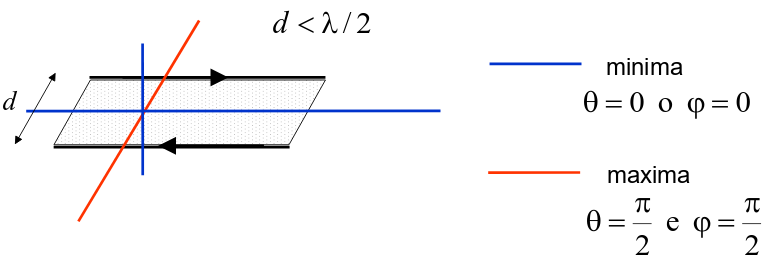
\includegraphics[width=0.6\linewidth]{immagini/emissioni_radiate17}
\end{figure}


Sotto la condizione geometrica consueta in cui la distanza tra le tracce sia inferiore a mezza lunghezza d'onda ($d < \lambda/2$), il campo elettrico massimo vale:
\[
E_{\text{max}} = \left| \vec{E}\left(r, \theta = \frac{\pi}{2}, \phi = \frac{\pi}{2}\right) \right| = -2j \vec{e}\left(\frac{\pi}{2}, \frac{\pi}{2}\right) I_{D0} \sin\left(\pi \frac{d}{\lambda}\right) \frac{e^{-j \beta r}}{r}
\]

L'entità dell'emissione radiata dipende criticamente dal parametro adimensionale $d/\lambda$, che quantifica la dimensione elettrica trasversale della linea:
\begin{itemize}
    \item \textbf{Condizione di perfetta cancellazione ($d/\lambda \to 0$)} $\rightarrow$ all'annullarsi della distanza elettrica, i contributi radiativi dei due conduttori si cancellano esattamente:
    \[
    \lim_{d/\lambda \to 0} E_{\text{max}} = 0
    \]
    \item \textbf{Emissione non intenzionale ($d/\lambda \ll 1$)} $\rightarrow$ sviluppando la funzione seno in serie di Taylor al primo ordine ($\sin(\pi d/\lambda) \approx \pi d/\lambda$):
    \[
    E_{\text{max}} \approx -2j \vec{e} I_{D0} \left(\pi \frac{d}{\lambda}\right) \frac{e^{-j \beta r}}{r}
    \]
    Il campo residuo non è nullo e cresce linearmente con la separazione fisica $d$.
    \item \textbf{Emissione intenzionale da antenna ($d/\lambda \to 1/2$)} $\rightarrow$ per $d = \lambda/2$, l'argomento del seno diviene $\pi/2$ e $\sin(\pi/2) = 1$:
    \[
    E_{\text{max}} \approx -2j \vec{e} I_{D0} \frac{e^{-j \beta r}}{r}
    \]
    I campi generati dalle due linee si sommano costruttivamente in opposizione spaziale, convertendo l'interconnessione in un'antenna efficiente.
\end{itemize}

L'evoluzione dei diagrammi di radiazione all'aumentare del rapporto $d/\lambda$ evidenzia tre scenari caratteristici per un conduttore di separazione $d = 1\text{ cm}$:
\begin{enumerate}
    \item Per $f = 300\text{ MHz}$ ($\lambda = 1\text{ m}$), si ha $d/\lambda = 0.01$: l'emissione è quasi interamente soppressa dall'interferenza distruttiva, con un lobo residuo estremamente compatto.
    \begin{figure}[H]
    	\centering
    	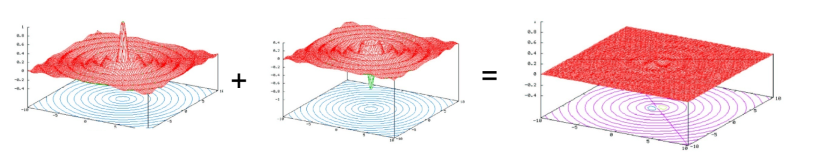
\includegraphics[width=0.9\linewidth]{immagini/emissioni_radiate18}
    \end{figure}
    \item Per $f = 3\text{ GHz}$ ($\lambda = 10\text{ cm}$), si ha $d/\lambda = 0.1$: la cancellazione parziale produce lobi di disturbo chiaramente definiti.
    \begin{figure}[H]
    	\centering
    	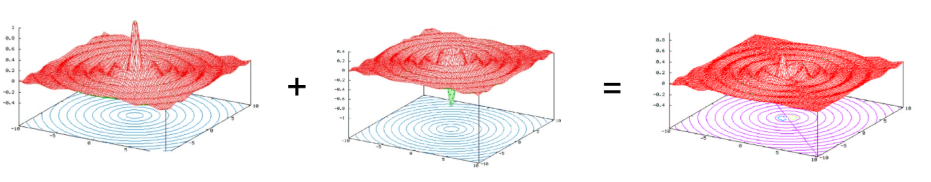
\includegraphics[width=0.9\linewidth]{immagini/emissioni_radiate19}
    \end{figure}
    \item Per $f = 15\text{ GHz}$ ($\lambda = 2\text{ cm}$), si ha $d/\lambda = 0.5$: la struttura si comporta a tutti gli effetti come un'antenna ad array, sviluppando lobi di radiazione ad alta direttività e massima efficienza di emissione.
    \begin{figure}[H]
    	\centering
    	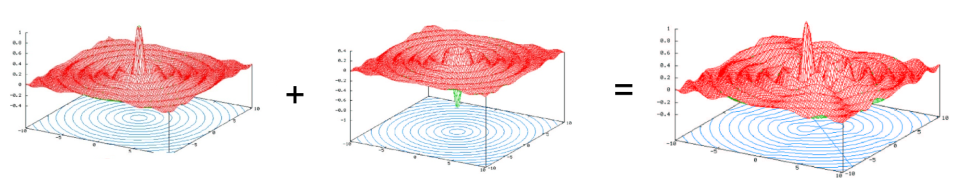
\includegraphics[width=0.9\linewidth]{immagini/emissioni_radiate20}
    \end{figure}
\end{enumerate}

Nel caso di linee elettricamente corte in senso longitudinale ($l \ll \lambda$), la distribuzione di corrente lungo il conduttore può essere considerata uniforme e costante:
\[
I_{D0}(z) \approx I_{D0} = \text{costante}
\]
Integrando il fattore di forma del dipolo corto e sostituendo $\beta = 2\pi f / v$, l'espressione del campo massimo irradiato nel vuoto assume la forma analitica:
\[
E_{\text{max}} = \frac{\mu \pi}{v} l d I_{D0} f^2 \frac{e^{-j \beta r}}{r}
\]
Sostituendo i valori numerici della permeabilità magnetica del vuoto $\mu_0 = 4\pi \cdot 10^{-7}\ \text{H/m}$ e della velocità della luce $c \approx 3 \cdot 10^8\ \text{m/s}$, il modulo del campo massimo vale:
\[
E_{\text{max}} = 1.316 \cdot 10^{-14} \frac{I_{D0} f^2 l d}{r}
\]

Dalla relazione si deducono i legami di proporzionalità che governano l'emissione di modo differenziale:
\begin{itemize}
    \item $E_{\text{max}}$ è direttamente proporzionale a:
    \begin{itemize}
        \item Livello di corrente di modo differenziale ($I_{D0}$).
        \item Quadrato della frequenza ($f^2$).
        \item Area della spira o maglia di circuito ($A = l \cdot d$).
    \end{itemize}
    \item $E_{\text{max}}$ è inversamente proporzionale a:
    \begin{itemize}
        \item Distanza dal punto di osservazione ($r$).
    \end{itemize}
\end{itemize}
\begin{figure}[H]
	\centering
	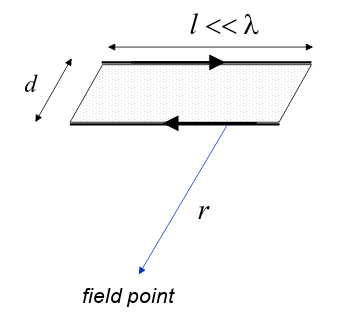
\includegraphics[width=0.35\linewidth]{immagini/emissioni_radiate21}
\end{figure}

Vediamo l'esempio di circuiti digitali pilotati da un segnale di clock:
\begin{figure}[H]
	\centering
	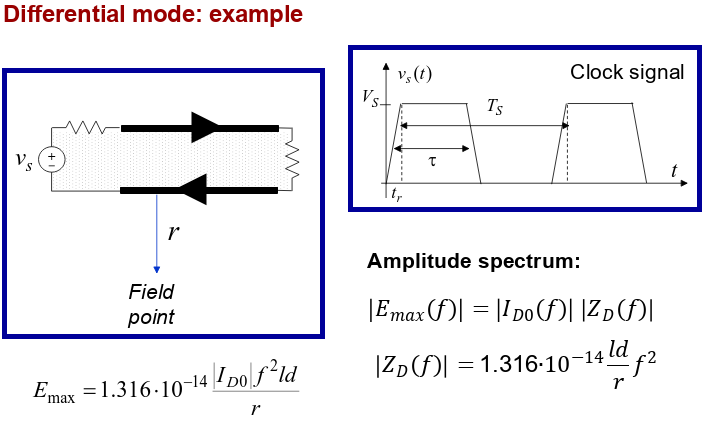
\includegraphics[width=0.8\linewidth]{immagini/emissioni_radiate22}
\end{figure}

Di seguito i diagrammi di Bode di $|Z_D(f)|$ e $|I_{D0}|$:
\begin{figure}[H]
	\centering
	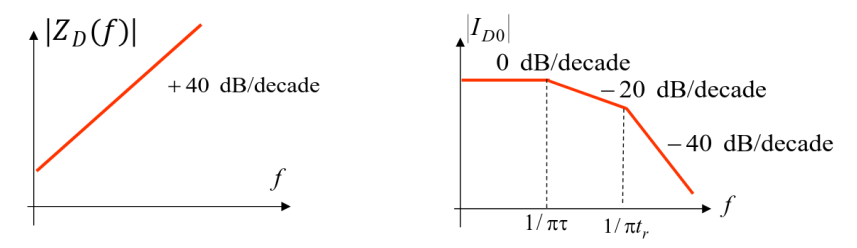
\includegraphics[width=0.7\linewidth]{immagini/emissioni_radiate23}
\end{figure}
La combinazione per somma logaritmica di questi, determina il profilo spettrale del campo elettrico radiato $E_{\text{max}}(f)$:
\begin{figure}[H]
	\centering
	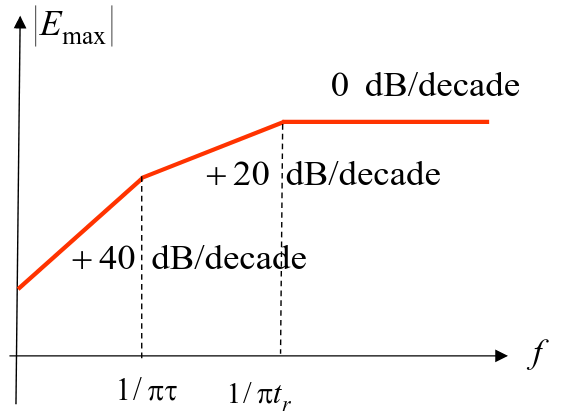
\includegraphics[width=0.3\linewidth]{immagini/emissioni_radiate24}
\end{figure}
A causa della dipendenza da $f^2$, lo spettro radiato di modo differenziale aumenta costantemente fino alla seconda frequenza di taglio, stabilizzandosi ad ampiezza costante ad alta frequenza senza esibire alcun decadimento spontaneo.

Le tecniche progettuali per la mitigazione delle emissioni radiate di modo differenziale derivano direttamente dalla proporzionalità $E_{\text{max}} \propto I_{D0} f^2 A$:
\begin{itemize}
    \item \textbf{Riduzione dell'ampiezza della corrente} $\rightarrow$ perseguibile attraverso:
    \begin{itemize}
        \item Riduzione della tensione di alimentazione del generatore $V_S$, poiché il livello di picco della corrente dipende dal rapporto $2 V_S / T_S$.
        \item Riduzione del duty cycle del segnale.
        \begin{figure}[H]
        	\centering
        	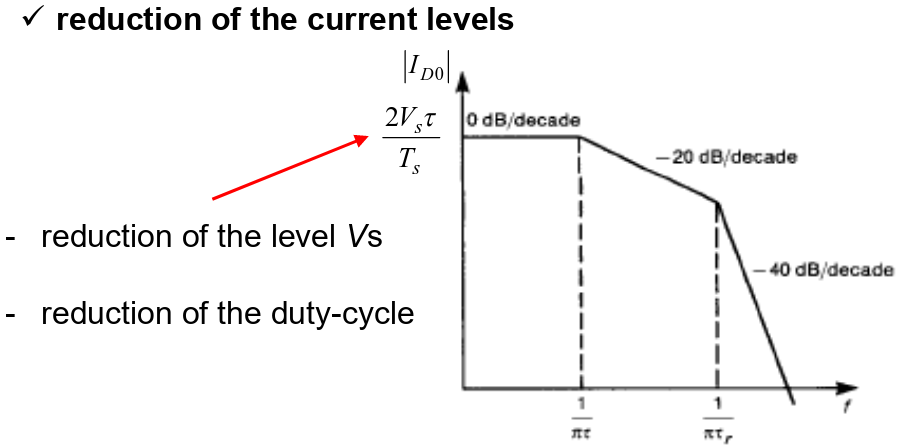
\includegraphics[width=0.5\linewidth]{immagini/emissioni_radiate25}
        \end{figure}
    \end{itemize}
    \item \textbf{Riduzione dell'area della maglia di circuito ($A = l \cdot d$)} $\rightarrow$ costituisce la misura di mitigazione più efficace, realizzabile tramite:
    \begin{itemize}
        \item Progettazione accurata del layout PCB: instradamento delle piste di andata e ritorno strettamente adiacenti o disposte parallelamente su strati adiacenti affacciati su un piano di massa continuo, minimizzando la distanza geometrica $d$.
        \item Scelta intelligente della piedinatura dei componenti (smart pinout): assegnazione contigua dei pin di segnale e dei rispettivi pin di ritorno di massa, evitando configurazioni con terminali opposti o dispersi che espandono l'area geometrica della spira.
    \end{itemize}
\end{itemize}
\begin{figure}[H]
	\centering
	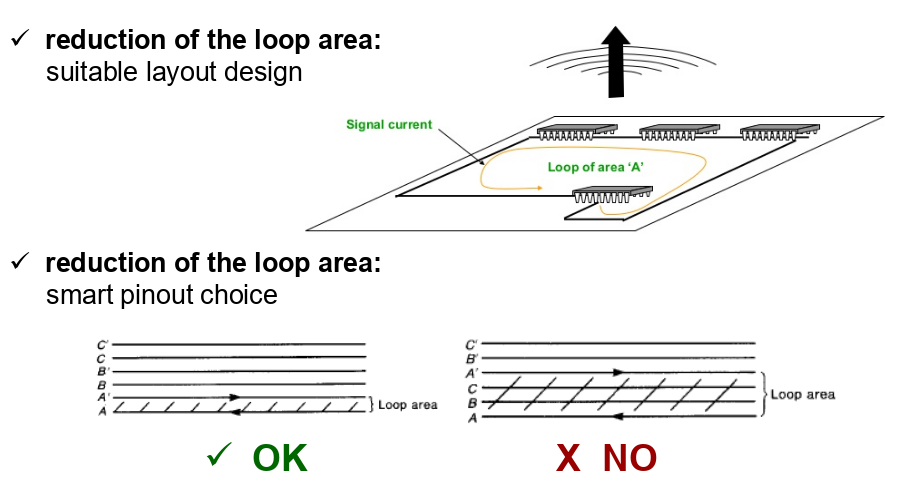
\includegraphics[width=0.7\linewidth]{immagini/emissioni_radiate26}
\end{figure}

\subsection{Emissione radiata di modo comune}
Nel regime di modo comune, le correnti lungo i due conduttori paralleli fluiscono nel medesimo verso con ampiezza concorde ($I_{01} = I_{C0}$, $I_{02} = I_{C0}$). 
\begin{figure}[H]
	\centering
	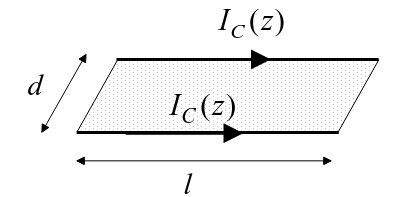
\includegraphics[width=0.3\linewidth]{immagini/emissioni_radiate27}
\end{figure}
Sostituendo tali grandezze nell'equazione di campo lontano:
\[
\vec{E} = \vec{e}(\theta, \phi) \frac{e^{-j \beta r}}{r} I_{C0} \left[ e^{-j \beta \Delta r} + e^{j \beta \Delta r} \right]
\]
Applicando le formule di Eulero per la funzione coseno, il campo elettrico radiato si esprime come:
\[
\vec{E} = 2 \vec{e}(\theta, \phi) \frac{e^{-j \beta r}}{r} I_{C0} \cos(\beta \Delta r)
\]
dove la variazione di fase è la medesima derivata in precedenza:
\[
\beta \Delta r = \pi \frac{d}{\lambda} \sin\phi \sin\theta
\]

L'analisi della funzione di modulazione spaziale $\cos(\beta \Delta r)$ evidenzia una proprietà fisica di rilievo primario:
\begin{itemize}
    \item \textbf{Minimi di emissione} $\rightarrow$ si ottengono nelle direzioni per cui l'argomento raggiunge $\beta \Delta r = \pi/2$.
    \item \textbf{Massimi di emissione} $\rightarrow$ si verificano per $\sin\phi = 0$ oppure $\sin\theta = 0$, dove $\beta \Delta r = 0$ e $\cos(0) = 1$. Il valore massimo del campo si colloca in direzione $\theta = \pi/2$ e $\phi = 0$:
    \[
    E_{\text{max}} = \left| \vec{E}\left(r, \theta = \frac{\pi}{2}, \phi = 0\right) \right| = 2 \vec{e}\left(\frac{\pi}{2}, 0\right) I_{C0} \frac{e^{-j \beta r}}{r}
    \]
\end{itemize}
\begin{figure}[H]
	\centering
	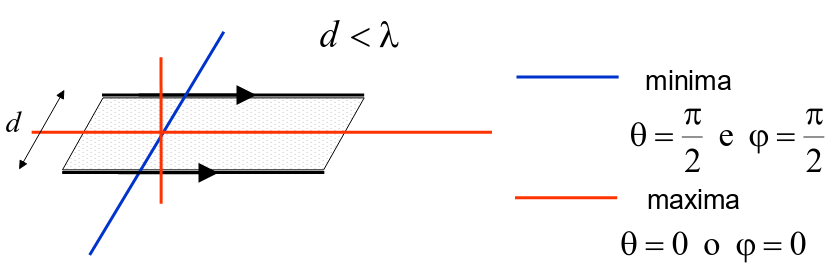
\includegraphics[width=0.5\linewidth]{immagini/emissioni_radiate28}
\end{figure}


A differenza di quanto accade per il modo differenziale, l'emissione di modo comune non si annulla affatto quando la separazione elettrica tende a zero ($d/\lambda \to 0$):
\[
\lim_{d/\lambda \to 0} \cos\left(\pi \frac{d}{\lambda} \sin\phi \sin\theta\right) = 1
\]
Ne consegue che, anche per valori estremamente bassi di $d/\lambda$ (ad esempio $d/\lambda = 0.01$ con $d = 1\text{ cm}$ e $f = 300\text{ MHz}$), i contributi radiativi generati dai due conduttori si sommano in fase in modo interamente costruttivo. La radiazione complessiva equivale al doppio del campo irradiato da un singolo conduttore isolato, e non beneficia di alcun meccanismo spontaneo di cancellazione spaziale.
\begin{figure}[H]
	\centering
	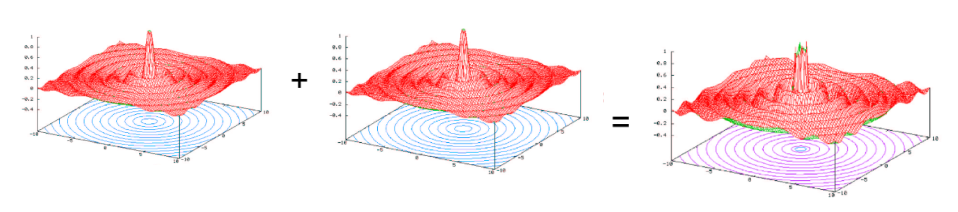
\includegraphics[width=0.9\linewidth]{immagini/emissioni_radiate29}
\end{figure}

Nel caso di interconnessioni corte rispetto alla lunghezza d'onda ($l \ll \lambda$), la corrente di modo comune può essere considerata uniforme lungo la coordinata $z$:
\[
I_{C0}(z) \approx I_{C0} = \text{costante}
\]
L'integrazione del modello per dipolo corto nel vuoto fornisce l'espressione analitica del campo massimo radiato:
\[
E_{\text{max}} = \mu \frac{l}{v} I_{C0} f \frac{e^{-j \beta r}}{r}
\]
Sostituendo i valori numerici della permeabilità del vuoto $\mu_0 = 4\pi \cdot 10^{-7}\ \text{H/m}$ e della velocità di propagazione, il valore assoluto del campo massimo si riduce alla formula semplificata:
\[
E_{\text{max}} = 1.257 \cdot 10^{-6} \frac{I_{C0} f l}{r}
\]

Dalla formula emergono i parametri che controllano l'emissione di modo comune:
\begin{itemize}
    \item $E_{\text{max}}$ è direttamente proporzionale a:
    \begin{itemize}
        \item Livello di corrente di modo comune ($I_{C0}$).
        \item Frequenza di lavoro ($f$, con andamento lineare e non quadratico).
        \item Lunghezza fisica del circuito o dell'interconnessione ($l$).
    \end{itemize}
    \item $E_{\text{max}}$ è inversamente proporzionale a:
    \begin{itemize}
        \item Distanza dal punto di osservazione ($r$).
    \end{itemize}
\end{itemize}
\begin{figure}[H]
	\centering
	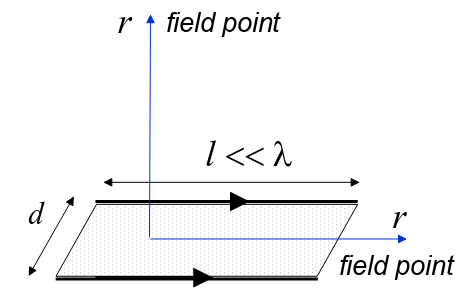
\includegraphics[width=0.4\linewidth]{immagini/emissioni_radiate30}
\end{figure}

Si osservi che l'emissione di modo comune non dipende in prima approssimazione dalla distanza trasversale $d$, bensì unicamente dalla lunghezza complessiva $l$ del conduttore.

Valutando nuovamente l'esempio di un segnale di clock:
\begin{figure}[H]
	\centering
	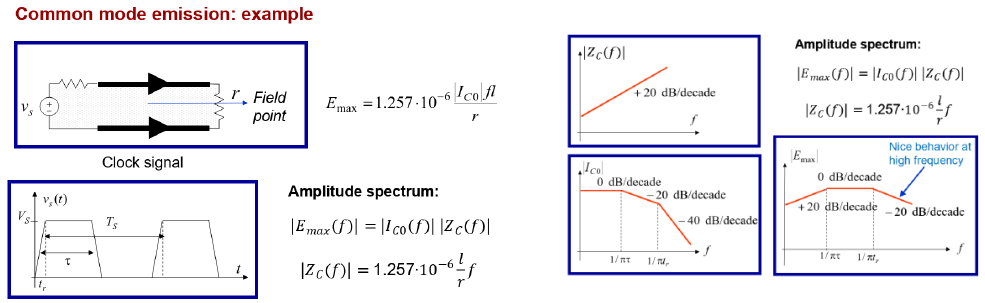
\includegraphics[width=1\linewidth]{immagini/emissioni_radiate34}
\end{figure}

Rispetto al modo differenziale, il modo comune presenta un comportamento intrinsecamente favorevole alle frequenze elevate: superata la frequenza d'angolo $1/(\pi t_r)$, il campo elettrico radiato decade con pendenza negativa pari a $-20\ \text{dB/decade}$, attenuando progressivamente il disturbo ad alta frequenza.

I criteri di contenimento dell'emissione di modo comune si articolano in due direttrici operative:
\begin{itemize}
    \item \textbf{Riduzione dei livelli di corrente} $\rightarrow$ a differenza della corrente differenziale, che convoglia il segnale informativo utile e non può essere soppressa, la corrente di modo comune costituisce un parametro parassita; in linea teorica, essa può e deve essere completamente eliminata mediante opportuno bilanciamento circuitale e disaccoppiamento.
    \item \textbf{Riduzione della lunghezza delle interconnessioni ($l$)} $\rightarrow$ attuabile collocando il generatore di clock il più vicino possibile ai moduli circuitali che ne richiedono la ricezione, riducendo al minimo geometrico lo sviluppo longitudinale delle piste.
    \begin{figure}[H]
    	\centering
    	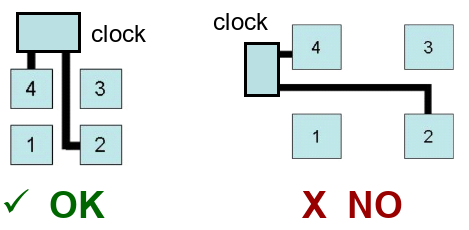
\includegraphics[width=0.35\linewidth]{immagini/emissioni_radiate33}
    \end{figure}
\end{itemize}

\subsection{Confronto tra modo comune e modo differenziale}
Il confronto tra i modelli analitici delle due modalità di emissione evidenzia differenze marcate sia nelle dipendenze fisiche sia nell'efficienza quantitativa di radiazione:
\begin{itemize}
    \item \textbf{Emissione di modo differenziale}:
    \[
    E_{\text{max}} = 1.316 \cdot 10^{-14} \frac{I_{D0} f^2 A}{r}
    \]
    Dipende quadraticamente dalla frequenza ($f^2$) e proporzionalmente all'area della spira ($A = l \cdot d$).
    \item \textbf{Emissione di modo comune}:
    \[
    E_{\text{max}} = 1.257 \cdot 10^{-6} \frac{I_{C0} f l}{r}
    \]
    Dipende linearmente dalla frequenza ($f^1$) e proporzionalmente alla sola lunghezza lineare del conduttore ($l$), risultando insensibile alla distanza $d$.
\end{itemize}

Il fattore numerico del modo comune ($1.257 \cdot 10^{-6}$) risulta superiore di circa otto ordini di grandezza rispetto al coefficiente del modo differenziale ($1.316 \cdot 10^{-14}$). Di conseguenza, livelli estremamente modesti di corrente parassita di modo comune sono in grado di produrre campi elettromagnetici radiati di entità comparabile o di gran lunga superiore rispetto a correnti differenziali di ampiezza considerevole.

L'effetto è quantificato analiticamente attraverso due casi di studio numerici, nei quali si calcolano i valori di corrente necessari a generare un campo limite prefissato pari a $E_{\text{max}} = 100\ \mu\text{V/m}$ alla distanza di misura normata $r = 3\text{ m}$, assumendo una spaziatura tra i conduttori $d = 1.27\text{ mm}$:
\begin{itemize}
    \item \textbf{Caso 1: interconnessione lunga a media frequenza} ($l = 1\text{ m}$, $f = 30\text{ MHz}$):
    \begin{itemize}
        \item Corrente di modo differenziale richiesta per generare $100\ \mu\text{V/m}$:
        \[
        I_D = 20\ \text{mA}
        \]
        \item Corrente di modo comune richiesta per generare il medesimo campo di $100\ \mu\text{V/m}$:
        \[
        I_C = 8\ \mu\text{A}
        \]
    \end{itemize}
    In questo scenario, la corrente di modo comune necessaria a superare la soglia di disturbo risulta 2500 volte inferiore rispetto alla corrente di modo differenziale.
    \item \textbf{Caso 2: interconnessione corta ad alta frequenza} ($l = 1\text{ cm} = 0.01\text{ m}$, $f = 300\text{ MHz}$):
    \begin{itemize}
        \item Corrente di modo differenziale richiesta per generare $100\ \mu\text{V/m}$:
        \[
        I_D = 20\ \text{mA}
        \]
        \item Corrente di modo comune richiesta per generare il medesimo campo di $100\ \mu\text{V/m}$:
        \[
        I_C = 80\ \mu\text{A}
        \]
    \end{itemize}
    Anche su tratti di linea di dimensioni centimetriche, sono sufficienti appena $80\ \mu\text{A}$ di corrente di modo comune per eguagliare l'effetto radiativo di una corrente differenziale di $20\ \text{mA}$ (rapporto pari a 250 a 1).
\end{itemize}

I risultati dei due casi di confronto sono riassunti nella tabella seguente:
\begin{center}
\begin{tabular}{|l|c|c|c|c|c|}
\hline
\textbf{} & \textbf{Lunghezza $l$} & \textbf{Frequenza $f$} & \textbf{Campo limite $E_{\text{max}}$} & \textbf{Corrente $I_D$} & \textbf{Corrente $I_C$} \\
\hline
Caso 1 & $1\ \text{m}$ & $30\ \text{MHz}$ & $100\ \mu\text{V/m}$ & $20\ \text{mA}$ & $8\ \mu\text{A}$ \\
\hline
Caso 2 & $1\ \text{cm}$ & $300\ \text{MHz}$ & $100\ \mu\text{V/m}$ & $20\ \text{mA}$ & $80\ \mu\text{A}$ \\
\hline
\end{tabular}
\end{center}

Tale disparità quantitativa dimostra in modo inequivocabile che, nella pratica della compatibilità elettromagnetica, i fallimenti delle prove di certificazione radiata sono quasi sistematicamente imputabili a correnti parassite di modo comune non previste in sede di progetto funzionale.

\section{Radiazione in campo lontano da spira di corrente}
La modellazione della radiazione da spira elementare di corrente consente di convalidare e generalizzare i risultati ottenuti per la coppia di conduttori in modo differenziale. Si consideri una spira chiusa planare (circolare o quadrata) di area geometrica $S$, collocata nell'origine delle coordinate e percorsa da una corrente stazionaria nel tempo di ampiezza $I_{S0}$.

Dalla teoria classica dell'elettromagnetismo, il momento di dipolo magnetico associato alla spira è definito da:
\[
m = I_{S0} S
\]
In condizioni di campo lontano ($r \gg \lambda$ e $r \gg \sqrt{S}$), i campi elettromagnetici irradiati presentano struttura completamente trasversa e assumono le espressioni:
\[
E_{\phi} = -j k \eta \frac{e^{-j k r}}{4\pi r} m k \sin\theta
\]
\[
H_{\theta} = j k \frac{e^{-j k r}}{4\pi r} m k \sin\theta
\]
dove $k = \beta = 2\pi/\lambda$ rappresenta il vettore d'onda e $\eta = \zeta$ è l'impedenza caratteristica del mezzo.

Valutando il massimo dell'ampiezza sul piano equatoriale ($\theta = \pi/2$) e sostituendo i parametri caratteristici dello spazio libero, il valore massimo del campo elettrico radiato nel vuoto a frequenza $f$ alla distanza $r$ è pari a:
\[
E_{\text{max}} = 1.316 \cdot 10^{-14} \frac{I_{S0} f^2 S}{r}
\]

Il campo radiato in campo lontano da una spira elementare di corrente presenta una struttura algebrica e funzionale del tutto identica a quella ricavata per la coppia di conduttori rettilinei alimentata da una corrente di modo differenziale, in cui l'area della spira $S$ corrisponde esattamente all'area della maglia formata dai conduttori di andata e ritorno ($S = l \cdot d$). Questo risultato conferma che ogni maglia circuitale chiusa percorsa da segnali differenziali agisce fisicamente nello spazio come una piccola antenna a dipolo magnetico, la cui efficienza di irradiazione scala proporzionalmente all'area racchiusa e al quadrato della frequenza operativa.
\begin{figure}[H]
	\centering
	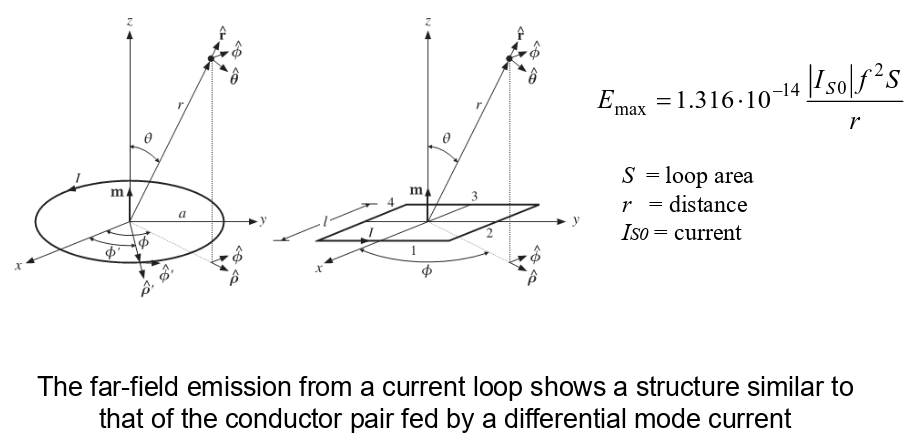
\includegraphics[width=0.8\linewidth]{immagini/emissioni_radiate35}
\end{figure}
